\chapter{Klassenbeschreibung}

\begin{figure}[ht]
    \centering
    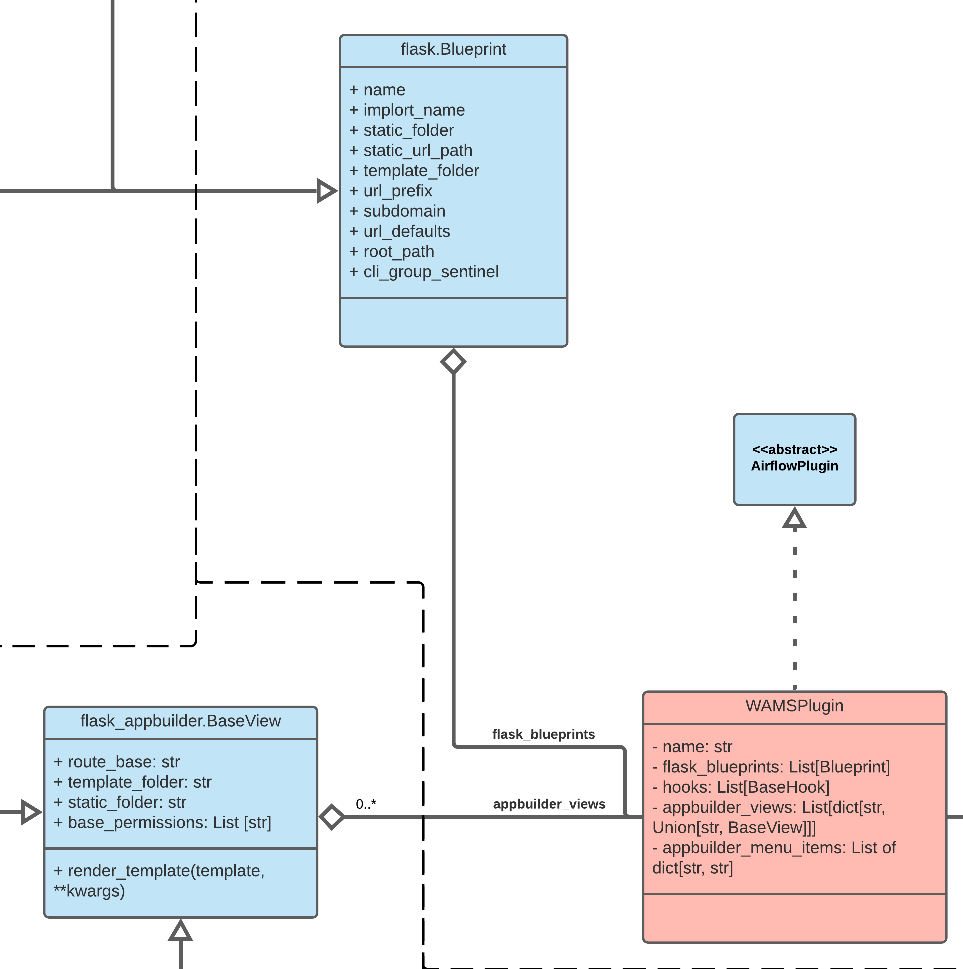
\includegraphics[width=\textwidth]{Diagramme/KlassendiagrammAusschnitte/Klassendiagramm - wamsplugin.png}
    \caption{Wams package}
    \label{fig:WamsPlugin}
\end{figure}

\subsection{WAMSPlugin}
Main Class of the WAMS Plugin for Airflow. Ties together the new views, functions and operators added in the plugin and implements the AirflowPlugin interface.
%Wrapper Klasse die die Hauptlogik des Plugins enthält und das AirflowPlugin interface implementiert.

\subsection{WAMSConfig}
Utility class that holds a dictionary of key value pairs, that represent the configuration of
WAMS. By default it loads the configuration stored in \verb!default_config.yaml!. An Config
singelton object is created during the initialisation of the application and its values are 
accessed via getter and setter methods to validate the inputs.
%Config datei siehe Daniel

\section{code\_editor}
\begin{figure} [ht]
    \centering
    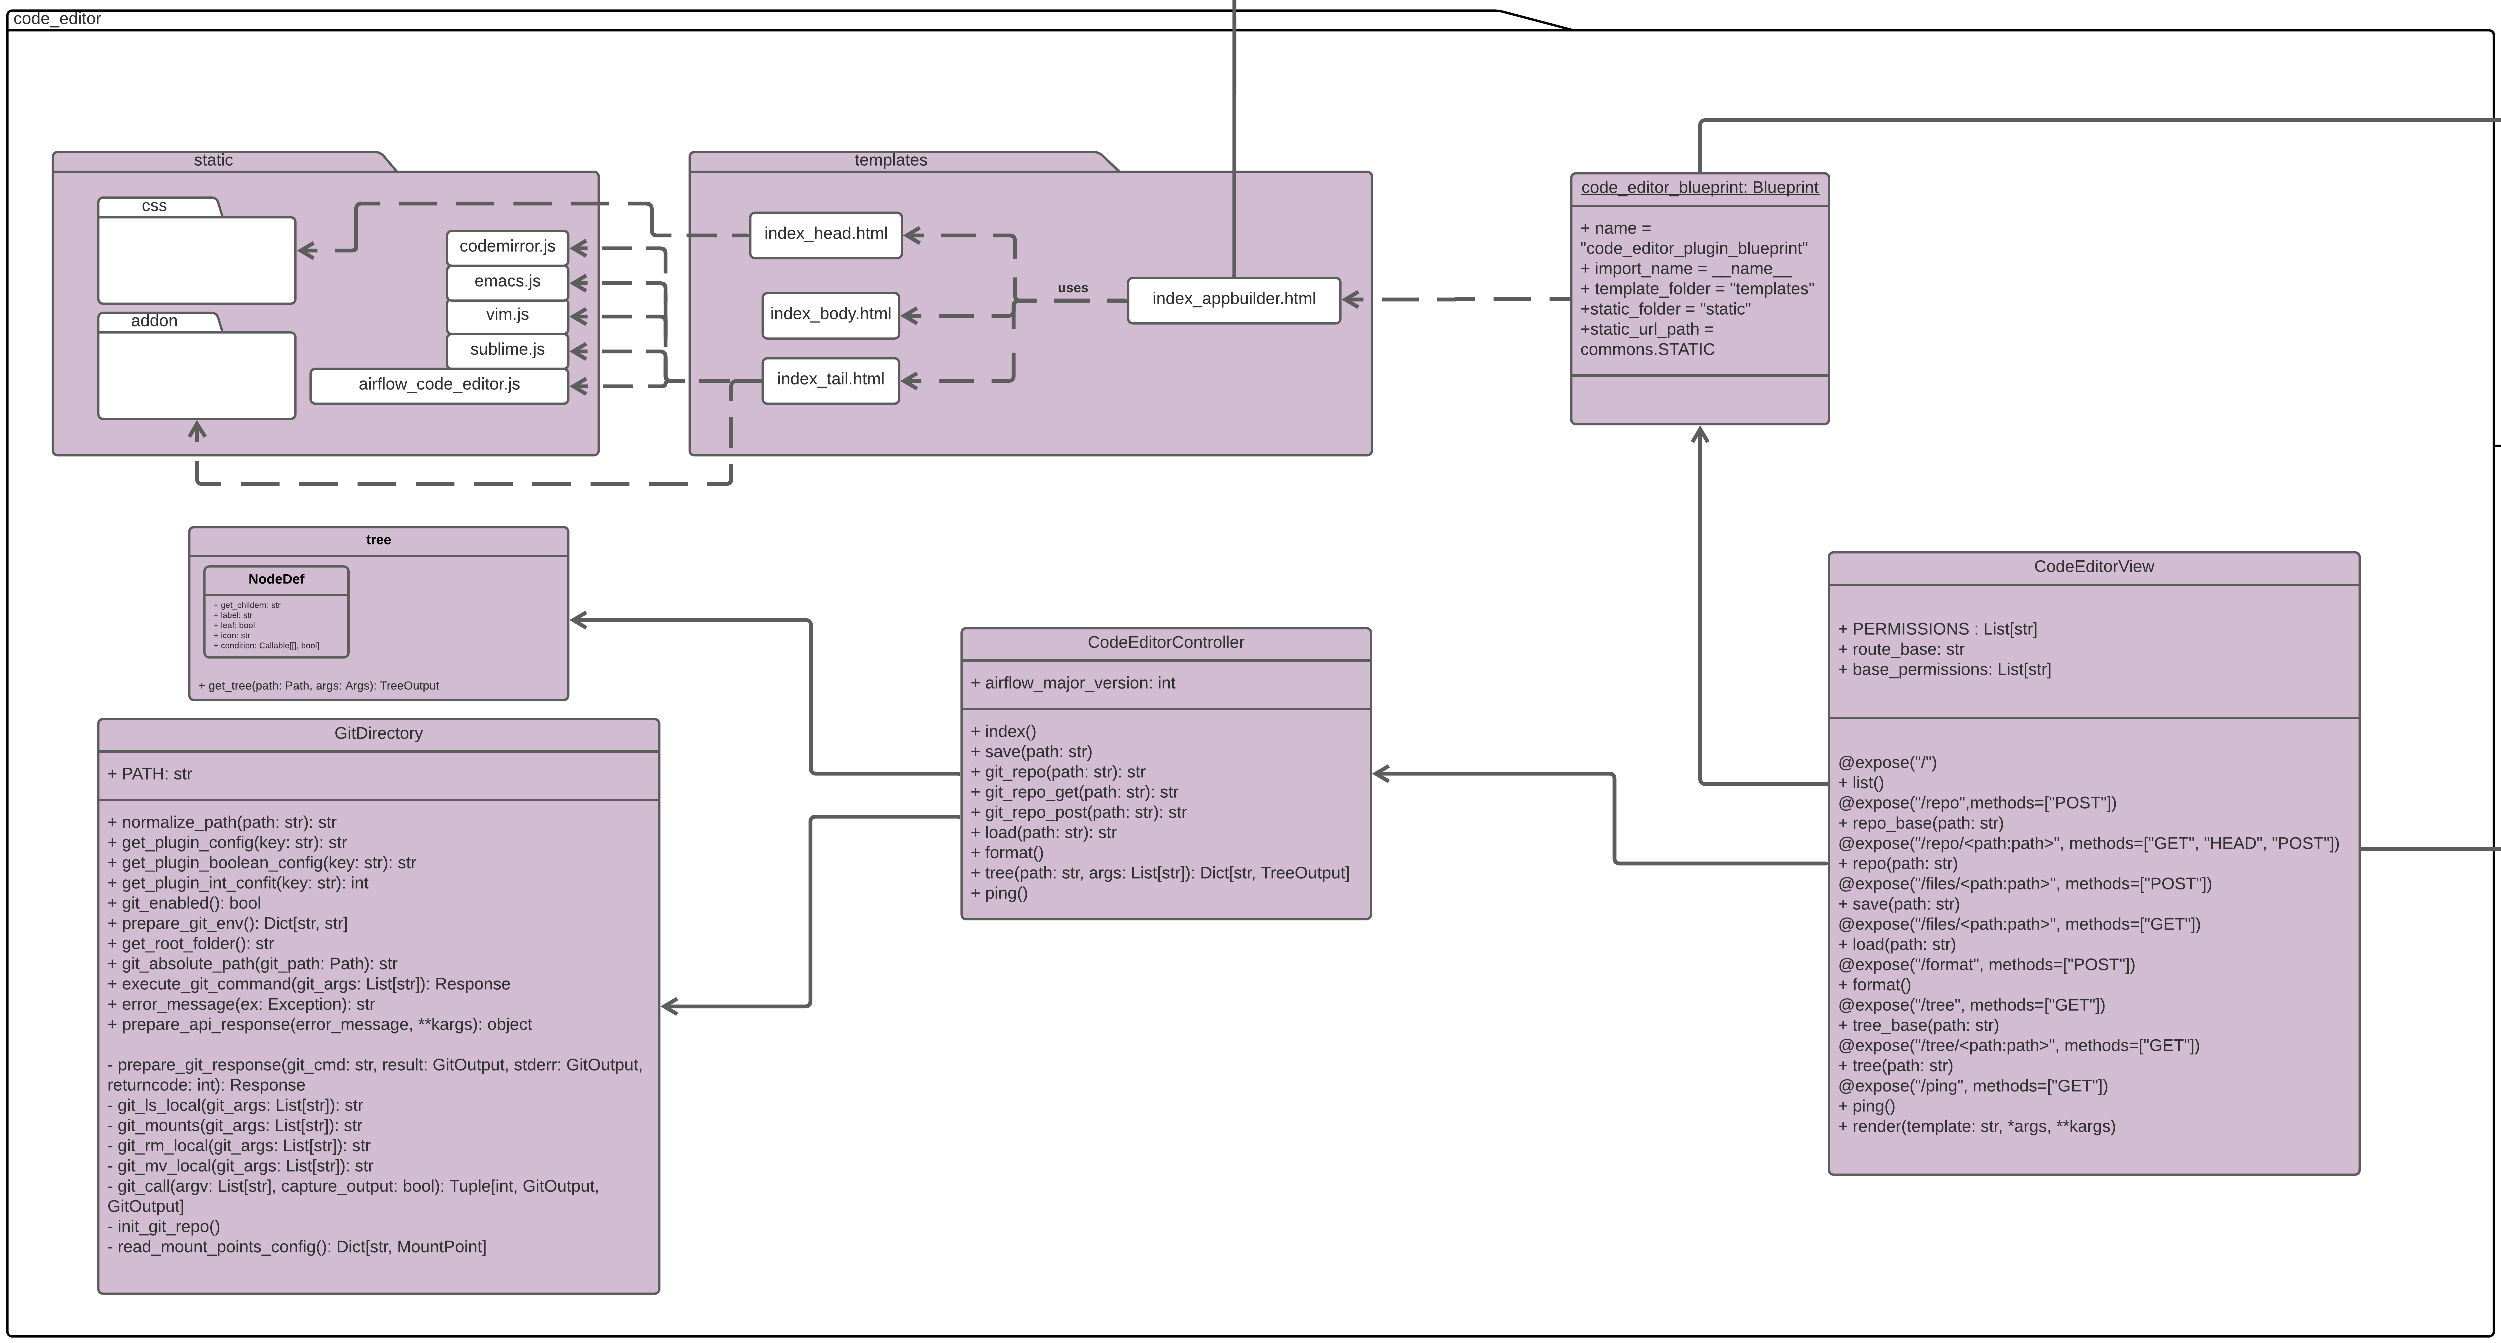
\includegraphics[width= \textwidth]{Diagramme/KlassendiagrammAusschnitte/Klassendiagramm -codeEditor.png}
    \caption{CodeEditor package}
    \label{fig:codeEditor section}
\end{figure}

\subsection{CodeEditorView}
Extends the flask\_appbuilder.BaseView class and handles the frontend of the CodeEditor package.
The CodeEditor view is added according to the Flask-AppBuilder Framework, that is used by Airflow for its Web-UI. It restricts access to the Editor according to the permissions and exposes the necessary URL-paths.

\subsection{CodeEditorController}
Implements the necessary logic for CodeEditorView and fetches the required data from GitDirectory, 
Tree.py and the dags directory.  

\subsection{code\_editor\_blueprint:Blueprint}
Flask blueprint used to handle the look and feel of the CodeEditor view.

\subsection{GitDirectroy}
Initializes and manages the git repository of the \verb!dags! folder. It
provides various methods to execute specific git commands on the git repository. 

\subsection{code\_editor.templates}
Templates folder for the code\_editor\_blueprint containing HTML files that determine the look of the CodeEditor view.

\subsection{code\_editor.static}
Static folder for the code\_editor\_blueprint containing CSS and JS files that determine the look and 
behavior of the CodeEditor view. It contains the files necessary for CodeMirror, directory and git view.

\subsection{tree}
Utility-class that is used by CodeEditorController to represent a file tree or git directory.


\subsection{results\_view\_blueprint:Blueprint}
Flask blueprint used to handle the look and feel of the Results view.


\section{metrics\_explorer}
Damit Nutzer von Airflow eine Übersicht über Metadaten von allen bereits ausgeführten Workflow Instanzen haben, fügt WAMS eine weitere Ansicht dafür hinzu.

 \begin{figure} [ht]
    \centering
    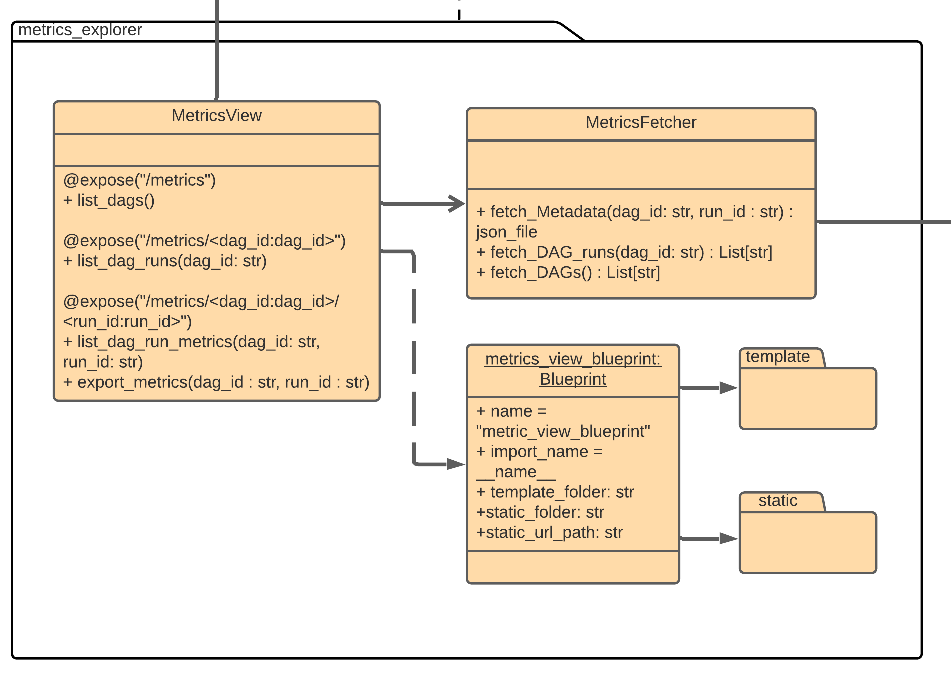
\includegraphics[width=\textwidth]{Diagramme/KlassendiagrammAusschnitte/Klassendiagramm -metadata explorer.png}
    \caption{Metadata package}
    \label{fig:metadata section}
\end{figure}


\subsection{MetricsView}
Extends flask\_appbuiler.BaseView to add a new view to the Webinterface of Airflow. It manages the
access rights and the frontend of the Metrics view.
%to write

\subsubsection{+ list\_dags()}
Lists all workflows in the current Airflow instance so that the user can select one of them.
The MetricsView gets the list from a MetricsFetcher instance.
\subsubsection{+ list\_dag\_runs(dag\_id: str)}
Lists all instances of a workflow that was just selected so that the user can select one of them.
It gets its the list from a MetricsFetcher instance.
\subsubsection{+ list\_dag\_run\_metrics(dag\_id: str, run\_id: str)}
Displays the metadata of the selected workflow instance.
It gets the metadata in form of a Json file from a MetricsFetcher instance.

\subsection{MetricsFetcher}
Fetches the required data for MetricsView from the WAMS Database. It converts the specific 
requests from MetricsView into API calls.

\subsubsection{+ fetchMetadata(dag\_id: str, run\_id) : json\_file}
Creates a json file from the response of the WAMS Database api calls and returns the that file.

%
%\subsection{JsonView}
%Responsible for formatting JSON files that are generated by MetricsFetcher. 

%\subsubsection{+ <<create>> \_\_init\_\_(file: json\_file)}
%Creates a new JsonView 

%\subsubsection{+ results(): json}
%Formats a JSON file making sure that the metadata is consistantly displayed.

%\subsubsection{+ download\_file()}
%Triggers the download of the formated JSON file.
%

\subsection{metrics\_view\_blueprint:Blueprint}
Flask blueprint that specifies the files used to handle the look and feel of the Metrics view.

\subsection{metrics\_explorer.templates}
Templates folder for the metrics\_view\_blueprint containing HTML files that determine the look of Metrics view.


\subsection{metrics\_explorer.static}
Static folder for the code\_editor\_blueprint containing CSS and JS files that determine the look 
and behavior of the Metrics view.

\section{wams\_operators}
\begin{figure} [ht]
    \centering
    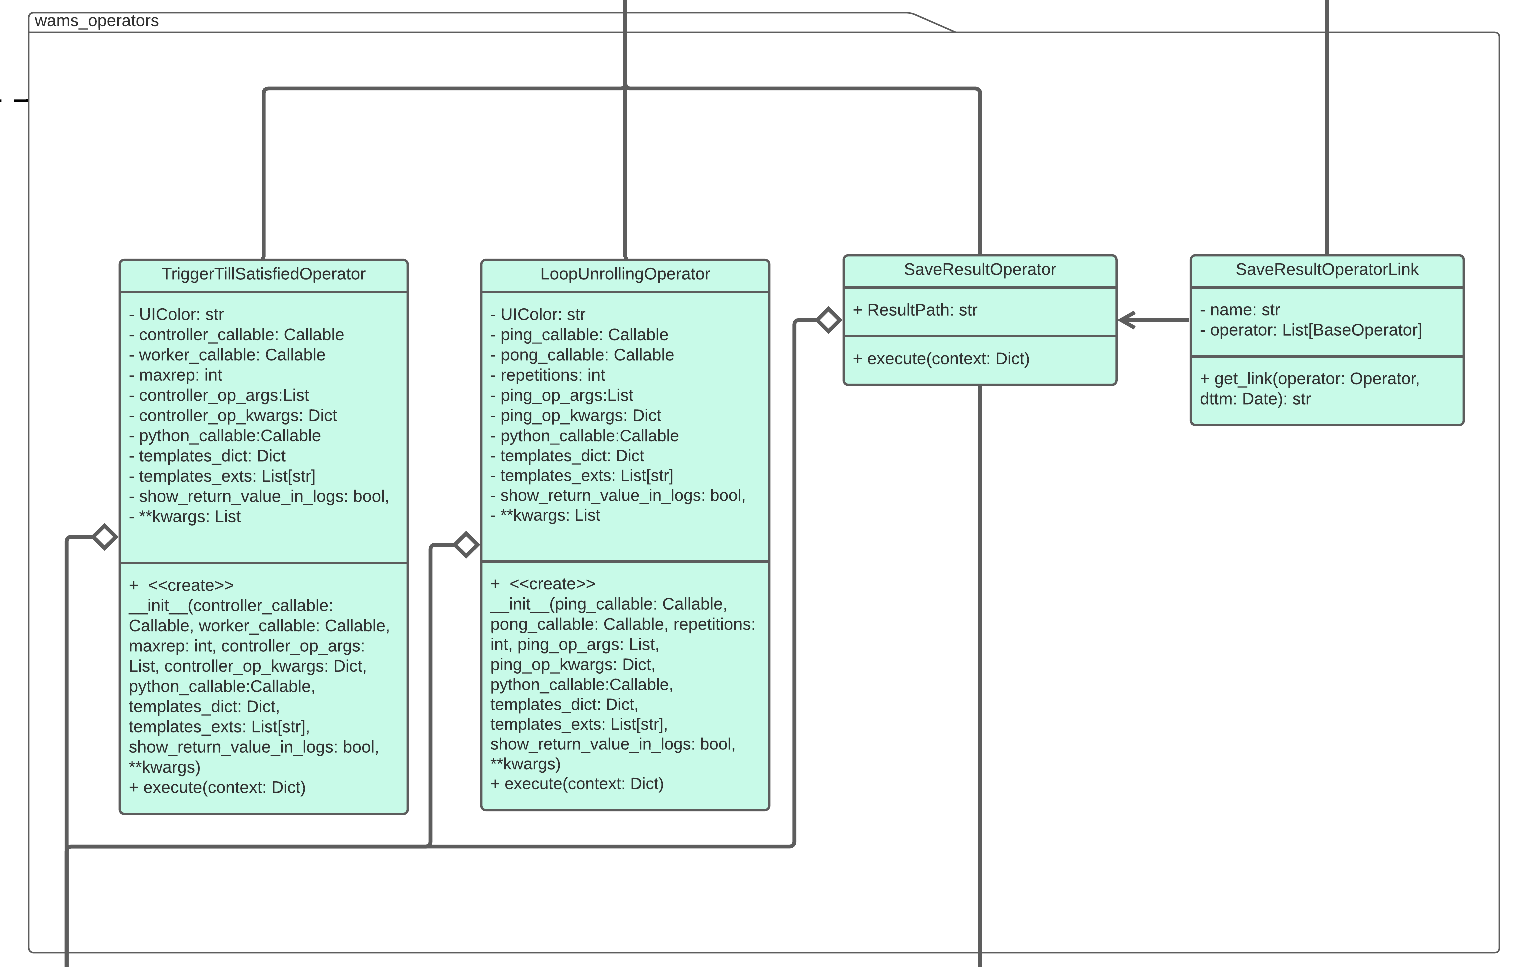
\includegraphics[width = \textwidth]{Diagramme/KlassendiagrammAusschnitte/Klassendiagramm -operators.png}
    \caption{Oparators package}
    \label{fig:operators section}
\end{figure}

\subsection{LoopUnrollingOperator}
%Operator class used for dynamically created tasks like the theory guided maschine learning modell.
This class represents an operator for Apache airflow and inherits from its base operator class.
The LoopUnrollingOperator receives two python callables. It executes both of them alternating as often as specified in the repetition parameter of its \textit{\_\_init\_\_()} method. The results of the callables can be used as input parameters for each repetition to allow to increase the accuracy of the model. The first callable can be started with parameters also passed via the \textit{\_\_init\_\_()} method.

\subsubsection{+  \_\_init\_\_(ping\_callable: Callable, pong\_callable: Callable, repetitions: int, ping\_op\_args: List, ping\_op\_kwargs: Dict, python\_callable:Callable, templates\_dict: Dict, templates\_exts: List[str], show\_return\_value\_in\_logs: bool, **kwargs: Dict)}

This method configures an instance of the LoopUnrollingOperator. In the parameters both callables and the number of repetitions must be parsed. Optional arguments like input parameters for the first callable execution can also be parsed.

\subsubsection{execute(context: Dict)} 
This method is derived from Airflows \textit{BaseOperator}-class. It initiates the execution of the task represented by the LoopUnrollingOperator.


\subsection{TriggerTillSatisfiedOperator}
This class represents an operator for Apache Airflow and inherits from its base operator class.
The TriggerTillSatisfiedOperator receives two python callables. In opposition to the \textit{LoopUnrollingOperator} the number of repetitions is not set via the \textit{\_\_init\_\_()} method but can change dynamically. The controller callable triggers the worker callable every time the worker has finished its work until the controller is satisfied with the result. To prevent to long runs a maximum of repetitions can also be passed in the \textit{\_\_init\_\_()} method. The controller callable receives the return values of the worker after every run of the worker.

\subsubsection{\_\_init\_\_(controller\_callable: Callable, worker\_callable: Callable, maxrep: int, controller\_op\_args: List, controller\_op\_kwargs: Dict, python\_callable:Callable,
templates\_dict: Dict, templates\_exts: List[str], show\_return\_value\_in\_logs: bool, **kwargs: Dict)}
This method configures an instance of the TriggerTillSatisfiedOperator. In the parameters the controller and worker callables must be parsed. Optional arguments like the maximum number of repetitions and input parameters for the controller can also be parsed.

\subsubsection{execute(context: Dict)} 
This method is derived from Airflows \textit{BaseOperator}-class. It initiates the execution of the task represented by the TriggerTillSatisfiedOperator.

\subsection{SaveResultOpertator}
This class represents an operator for Apache Airflow and inherits from its base operator class.
The main purpose of the SaveResultOperator is making the process of saving results, interim 
results and metadata as easy and uncomplicated as possible. The developer of a workflow should be able to save
results, interim results and metadata of his workflow by only adding this operator after a previous task 
which produced the result. The final storage control is not a part of this class but of the 
\textit{wams\_database} package.

\subsubsection{+ execute(context: Dict)} 
This method is derived from Airflows \textit{BaseOperator}-class. It saves the result or interim result of the workflow the SaveResultOperator belongs to in the current state of the workflow execution. 

\subsection{SaveResultOperatorLink}
This class creates a link which is added to every \textit{SaveResultOperator}. The link will be shown in the menu that pops up if the operator is clicked after a workflow was run. The link leads to the result view for the interim result or result stored by the \textit{SaveResultOperator} the SaveResultOperatorLink belongs to.

\subsubsection{+ get\_link(operator: Operator,  dttm: Date): str}
This method receives the operator the link for should be shown in and the date and time of its execution and returns a link. The operator should be a \textit{SaveResultOperator} and the link should lead directly to the result view for the result or interim result stored by this specific \textit{SaveResultOperator}.

\begin{figure} [h]
    \centering
    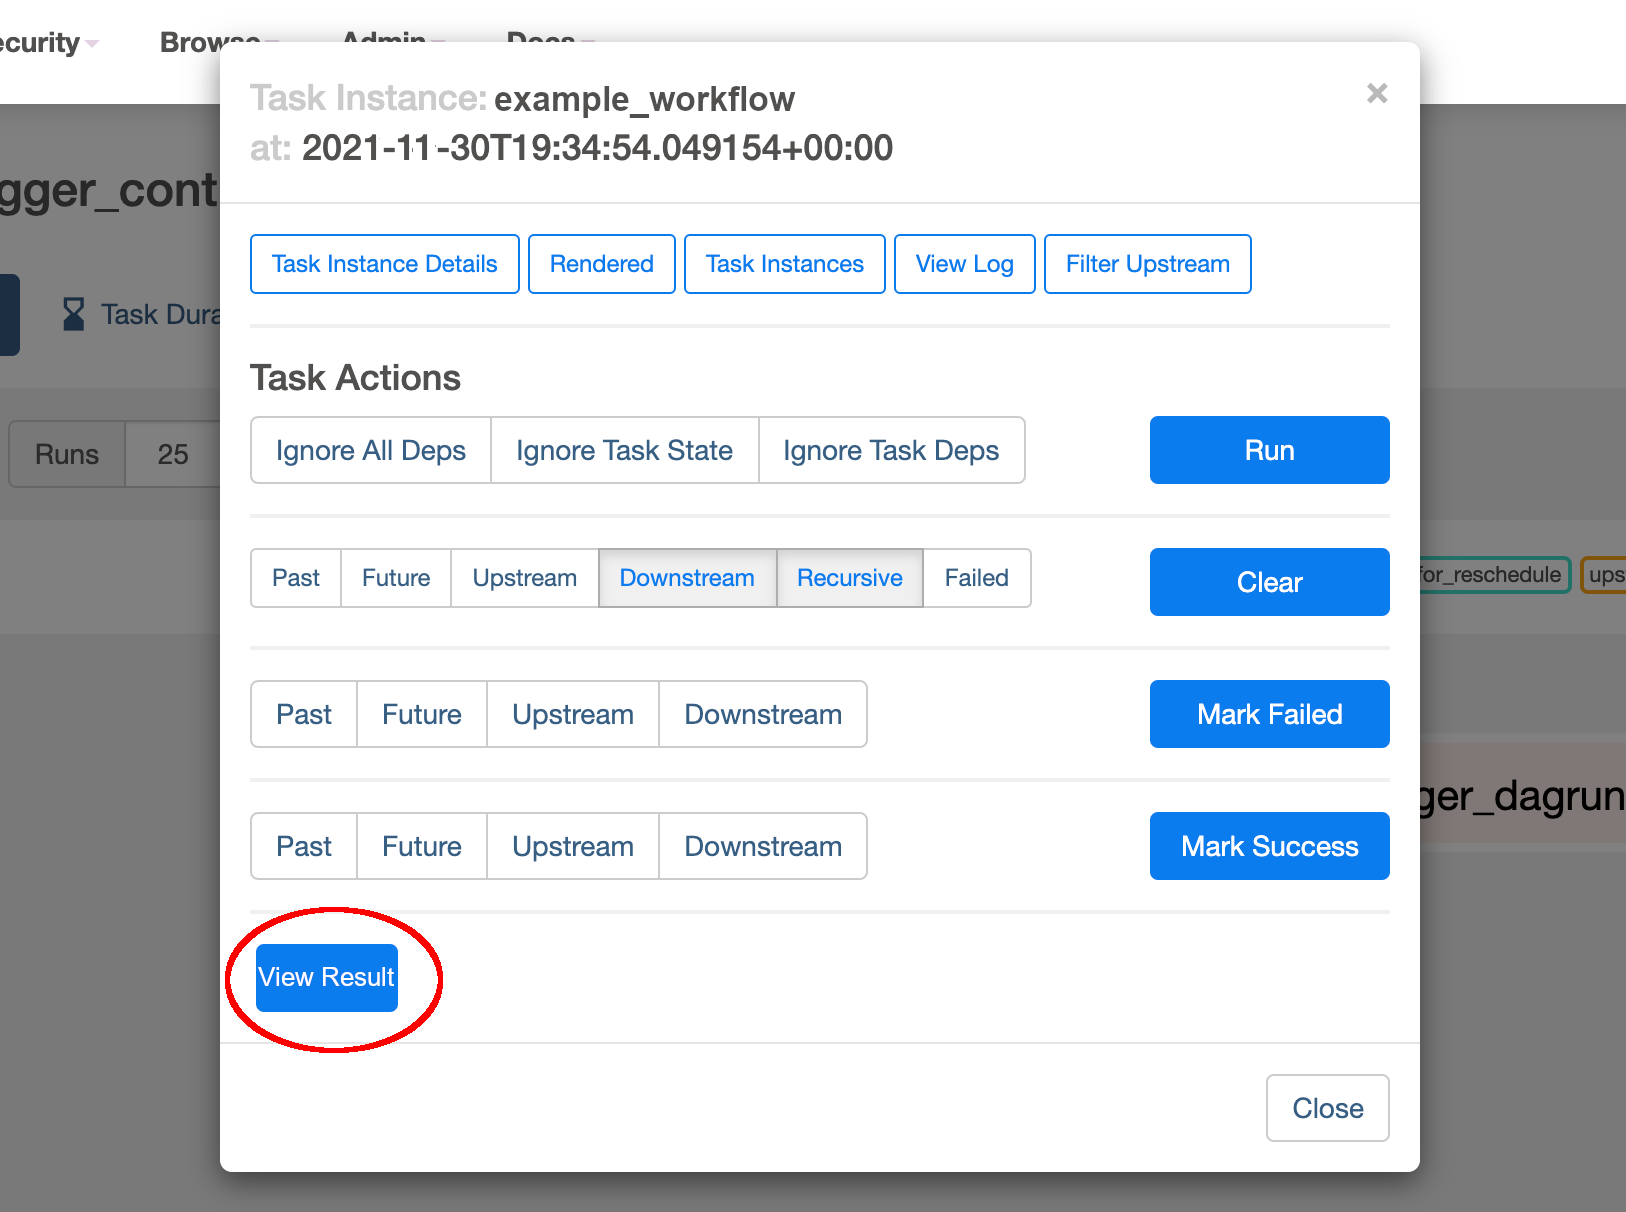
\includegraphics[width = 0.75\textwidth]{Grafiken/operator_extra_link.png}
    \caption{Beispielhafte Ansicht der Weboberfläche, wenn nach der Ausführung des Workflows \textit{example\_workflow} der SaveResultOperator angeklickt wurde. Die Klasse SaveResultOperatorLink sorgt dafür, dass der rot eingekreiste Button hinzugefügt wird}
    \label{fig:expSaveLink}
\end{figure}

\section{wams\_database}
Airflow bietet schon eine Datenbank, Metadaten bezüglich der einzelnen Workflows und den
ausgeführten Workflow Instanzen bietet. Jedoch bietet Airflow keine eigene Datenbank, die die
Ergebnisse von Workflows speichert. Um diese Funktionalität zu implementieren, hat WAMS eine
eigene Datenbank in einem separatem Container, die die Resultate, die über den SaveResultOperator gespeichert werden, speichert. %%%%%%TODO

\begin{figure} [ht]
    \centering
    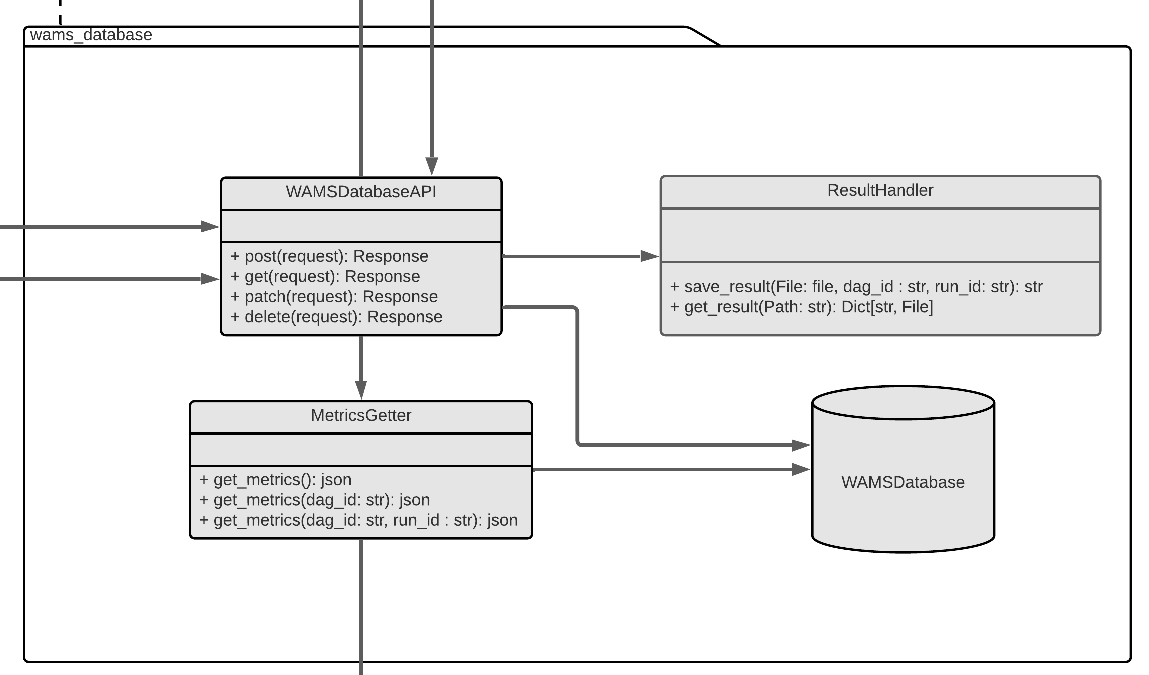
\includegraphics[width=0.9\textwidth]{Diagramme/KlassendiagrammAusschnitte/Klassendiagramm -database.png}
    \caption{Database package}
    \label{fig:database section}
\end{figure}

\subsection{WAMSDatabaseAPI}
Extends the rest\_framework.views.APIView to provide an API Django REST API for the other
parts of the WAMS-Plugin. The functions that this API handels are:
\begin{itemize}
    \item List all existing workflows and workflow instances
    \item Fetch the metadate for a particular workflow instance
    \item Upload a file generated by a workflow instance for persistent storage
    \item Fetch a file generated by a workflow instance to display it to the user
\end{itemize}
The WAMSDatabaseAPI class recognizes which action is requested and forwards the action to
the ResultHandler or MetricsGetter.

\subsubsection{+ post(request): Response}
Implementation of the POST endpoint of the Django RESTful API. This handles inserting new data into the WAMSDatabase and returns a response object depending on the outcome of the operation.
%Handles a POST request made to the API this class represents. 
\subsubsection{+ get(request): Response}
Implementation of the GET endpoint of the Django RESTful API. This handles getting data from the WAMSDatabase and returns a response object depending on the outcome of the operation.
%Handles a GET request made to the API this class represents.
\subsubsection{+ patch(request): Response}
Implementation of the PATCH endpoint of the Django RESTful API. This handles overwriting data within the WAMSDatabase and returns a response object depending on the outcome of the operation.
\subsubsection{+ delete(request): Response}
Implementation of the DELETE endpoint of the Django RESTful API. This handles removing data within the WAMSDatabase and returns a response object depending on the outcome of the operation.

\subsection{ResultHandler}
Handles the results generated by a workflow instance, that are uploaded via the
SaveResultOperator. Each file uploaded is stored in a directory according to the workflow
and the workflow instance that generated it.

\subsubsection{+ save\_result(File: file, dag\_id: str, run\_id: str): str}
Saves a given file in the results directory according to the dag\_id and run\_id so that they can
be retrieved for later use.
\subsubsection{+ get\_result(Path: str): Dict[str, File]}
Retrieves the results from a DAG run from the results directory according to the given path.


\subsection{MetricsGetter}
Handles the metadata generated by airflow for a workflow instance. When the metadata for a
workflow instance is requested it firstly polls the Airflow database over the Airflow API
for its data, if no data is found, it polls the WAMSDatabase for the data, since the workflow
might have been deleted.

\subsubsection{+ get\_metrics(): json}
Makes an API call to get a list of all workflows in airflow.

\subsubsection{+ get\_metrics(dag\_id: str): json}
Makes an API call to get a list of all workflow instances of a given workflow.

\subsubsection{+ get\_metrics(dag\_id: str, run\_id : str): json}
Makes an API call to get the metadata for a specific workflow instance.


\subsection{WAMSDatabase}
MySQL Database that persistently stores the results, interim results and the metadata for a workflow instance. After a workflow finishes and stores its results its metadata is fetched from the Airflow database and stored in this database to protect it from deletion after a workflow is deleted.
Results and interim results are stored into the database by the \textit{SaveResultOperator}.
%PPPPPaRamEteR spEiCherN?

\section{result\_view}

\begin{figure} [ht]
    \centering
    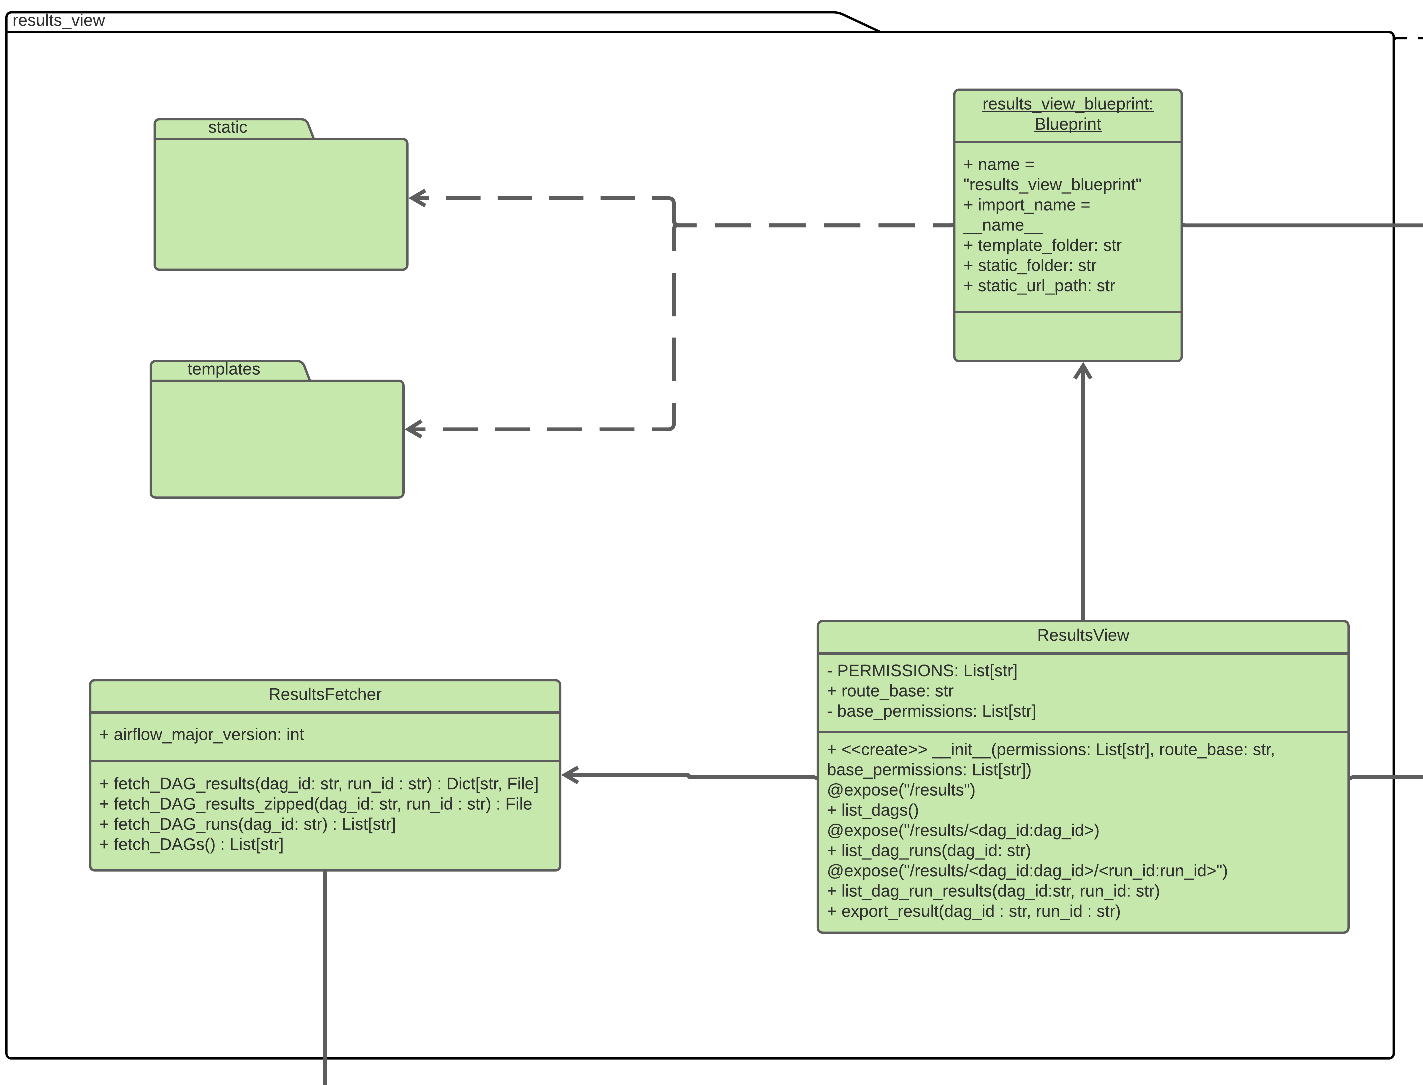
\includegraphics[width = \textwidth]{Diagramme/KlassendiagrammAusschnitte/Klassendiagramm -results view.png}
    \caption{Result\_view package}
    \label{fig:results section}
\end{figure}

\subsection{ResultsView}
Frontend for a AppBuilder view that lists all results generated and stored with the SaveResultOperator in the WAMSDatabase by the workflow and workflow instance that generated them.

\subsubsection{+ \_\_init\_\_(permissions: List[str], route\_base: str, base\_permissions: List[str]}
Creates a new ResultsView instance.

\subsection{+ list\_dags()}
Lists all workflows in the current Airflow instance so that the user can select one of them.
The ResultsView gets the list from a ResultsFetcher instance.

\subsubsection{+ list\_dag\_runs(dag\_id: str)}
Lists all instances of a workflow that was just selected so that the user can select one of them.
It gets its the list from a ResultsFetcher instance.

\subsubsection{+ list\_dag\_run\_results(dag\_id:str, run\_id: str)}
Displays the results of the selected workflow instance.
It gets the results from a ResultFetcher instance.

\subsubsection{+ export\_result(dag\_id : str, run\_id : str)}
Triggers the export of the results of a workflow instance.



\subsection{results\_view\_blueprint:Blueprint}
Flask blueprint used to handle the look and feel of the Results view.

\subsection{ResultsFetcher}
Backend for Results view that requests the required data from the WAMS Database over the network,
with the needed REST API calls.

\subsubsection{+ fetch\_DAG\_results(dag\_id: str, run\_id : str) : Dict[str, File]}
Constructs an API call to the WAMS Database that gets a list of all the files created by a 
given workflow instance.

\subsubsection{+ fetch\_DAG\_runs(dag\_id: str) : List[str]}
Constructs an API call to the WAMS Database that gets a list of all workflow instances that were created from a given workflow.

\subsubsection{+ fetch\_DAGs() : List[str]}
Constructs an API call to the WAMS Database that gets a list of all workflows in the Airflow database.

\subsection{result\_view.static}
Templates folder for the metrics\_view\_blueprint containing CSS and JS files that determine
the look and behavior of the Results view.

\subsection{result\_view.templates}
Templates folder for the metrics\_view\_blueprint containing HTML files that determine the 
look of the Results view.

\section{Externe Klassen} 
Klassen die nicht im Rahmen des Projekts entwickelt werden, aber trotzdem für den Aufbau relevant 
sind, da sie erweitert werden oder referenziert werden.

\subsection{AirflowPlugin}
Specifies the fields a plugin class must assign values to making Airflow able to import the Plugin.

\subsection{flask\_appbuilder.BaseView}
Base class from the Flask Appbuilder that declares the behaviour of a website created by Flask AppBuilder.

\subsection{BaseOperator}
Base class for workflow operators, that are then used in a workflow to be executed by the
Airflow worker.

\subsection{BaseOperatorLink}
Base class for classes that add a link to a workflow operator task page.

\subsection{Airflow API}
The REST API that Airflow exposes to access the various functions of the Airflow CLI. It also grants access to the metadata for workflow instances.

\subsection{List DAGs (resource)}
A list of all workflows in Airflow.

\subsection{List DAG runs (resource)}
A list of all workflow instances in Airflow.

\subsection{flask.Blueprint}
Class that specifies Flask which directories are to be used to specify the look and feel of a Website.

\subsection{appbuilder/general/model/list.html}
A HTML template from the Flask AppBuilder Framework.

\subsection{rest\_framework.views.APIView}
The base class for a Django REST API that handles the requests via its own implementation of pre-defined methods.

